\documentclass{CInf_practice}

% Rasmus,
% 3.3 habe ich anders gelöst. Wenn ich Zahlen schon weg habe, dann kümmere ich 
% mich nicht mehr um weitere Gruppen.
% Dadurch fällt z.B. die grüne Gruppe der DMF in b) raus, sowie bei der KMF
% das Quadrat cb und die Spalte ba. Danach bleiben:
% DMF: \comp a \comp d + \comp cd + c\comp d
%   (Alternativ: \comp a \comp c + \comp cd + c\comp d)
% KMF: (a + b + \comp d) \cdot (\comp c + \comp d)
%    = \comp a \comp c + DMF (obere)
%    oder
%    = \comp a \comp d + DMF (untere)
% -> Da die beiden DMFs ja durch ODER verknüpft werden können, müssen die 
% beiden also äquivalent sein.
% Die Truthtables zeigen das auch.
%
% Leider bin ich nicht clever genug, zu zeigen dass DMF + something = DMF ist.
%
% Viele Grüße
% Sebastian

\usepackage{multicol}

\usetikzlibrary{matrix}
\tikzstyle{highlight}=[densely dotted,line width=.7pt,draw,rounded corners=5pt]
\tikzstyle{matrix node}=[anchor=center,draw,shape=rectangle,text width=3em,minimum height=3em,text centered]

\sheet{3}{Schaltfunktionen und Minimierung}

\begin{document}

\cinftitle

\ex{Normalformen}{6 + 6 + 6 + 6 + 6 }
Anmerkung: Außer Duplikation von Termen wurde fast immer das 5. Axiom (vorwärts
oder rückwärts) zur Vereinfachung angewandt.

\begin{enumerate}[label=\alph{*})]
   \item
      \begin{equation*}
         f_{DKF} = \comp a\comp b \comp c + \comp a b\comp c + \comp a b c + 
         a b\comp c \\
      \end{equation*}
   \item
      \begin{eqnarray*}
         f_{DNF} & = & \comp a\comp b \comp c + \comp a b\comp c + \comp a b c + 
         a b\comp c \\
                 & = & \comp a \comp b \comp c + \comp a b \comp c + \comp a b
                       \comp c + \comp a b \comp c + \comp a b c + a b \comp c \\
                 & = & \comp a \comp c + b \comp c + \comp a b
      \end{eqnarray*}
   \item
      \begin{equation*}
         f_{KKN} = (a + b + \comp c) \cdot (\comp a + b + c) \cdot (\comp a
         + b  +\comp c) \cdot (\comp a + \comp b  +\comp c)
      \end{equation*}
   \item
      \begin{eqnarray*}
         f_{KKN} & = & (a + b + \comp c) \cdot (\comp a + b + c) \cdot (\comp a + b  +\comp c) \cdot (\comp a + \comp b  +\comp c) \\
                 & = & (a + b + \comp c) \cdot (\comp a + b + c) \cdot (\comp a
                        + b  +\comp c) \cdot (\comp a + \comp b  +\comp c) \cdot (\comp a + b + \comp c)\\
                 & = & (a + b + \comp c) \cdot ((\comp a + b) + (c\comp c)) \cdot ((\comp a + \comp c) + (b\comp b)) \\
                 & = & (a + b \comp c) \cdot (\comp a + b) \cdot (\comp a + \comp c) \\
                 & = & (\comp a + b) \cdot (\comp c + ((a + b)\cdot\comp a)) \\
                 & = & (\comp a + b) \cdot (\comp c + (a\comp a + \comp a b)) \\
                 & = & (\comp a + b) \cdot (\comp c + \comp a b) \\
                 & = & (\comp a + b) \cdot (\comp a + \comp c) \cdot (b + \comp c)
      \end{eqnarray*}

   \item \hspace{\linewidth} % weirdly, i must put space here in order for the
                             % tikzpicture to start at the next line

      \begin{center}
      \begin{tikzpicture}[node distance=.5cm,every node/.style={scale=.8}] % TODO: Encapsulate some of this stuff in macros
            \node (a) {$a$};
            \node[right=of a] (b) {$b$};
            \node[right=of b] (c) {$c$};
            \draw[name path=a-line](a) -- ++(0,-6cm);
            \draw[name path=b-line](b) -- ++(0,-6cm);
            \draw[name path=c-line](c) -- ++(0,-6cm);

            \node[and port, below right=.5cm and 2 cm of c] (and-1) {};
            \draw[name path=a-and-1] (a) |- (and-1.145);
            \draw[name path=b-and-1] (b) |- (and-1.180);
            \draw[name path=c-and-1] (c) |- (and-1.215);
            \fill[black,name intersections={of=a-line and a-and-1}] (intersection-1) circle (1.5pt);
            \fill[black,name intersections={of=b-line and b-and-1}] (intersection-1) circle (1.5pt);
            \fill[black,name intersections={of=c-line and c-and-1}] (intersection-1) circle (1.5pt);
            \begin{scope} % scope to only clip circles
               \clip (and-1.north west) rectangle ++(-3cm,-3cm); % to cut circles
               \node[shape=circle,draw,fill=white,inner sep=1.5pt,left=0pt of and-1.145] () {};
               \node[shape=circle,draw,fill=white,inner sep=1.5pt,left=0pt of and-1.180] () {};
               \node[shape=circle,draw,fill=white,inner sep=1.5pt,left=0pt of and-1.215] () {};
            \end{scope}

            % second and
            \node[and port, below=of and-1] (and-2) {};
            \draw[name path=a-and-2] (a) |- (and-2.145);
            \draw[name path=b-and-2] (b) |- (and-2.180);
            \draw[name path=c-and-2] (c) |- (and-2.215);
            \fill[black,name intersections={of=a-line and a-and-2}] (intersection-1) circle (1.5pt);
            \fill[black,name intersections={of=b-line and b-and-2}] (intersection-1) circle (1.5pt);
            \fill[black,name intersections={of=c-line and c-and-2}] (intersection-1) circle (1.5pt);
            \begin{scope} % scope to only clip circles
               \clip (and-2.north west) rectangle ++(-3cm,-3cm); % to cut circles
               \node[shape=circle,draw,fill=white,inner sep=1.5pt,left=0pt of and-2.145] () {};
               \node[shape=circle,draw,fill=white,inner sep=1.5pt,left=0pt of and-2.215] () {};
            \end{scope}

            % third and
            \node[and port, below=of and-2] (and-3) {};
            \draw[name path=a-and-3] (a) |- (and-3.145);
            \draw[name path=b-and-3] (b) |- (and-3.180);
            \draw[name path=c-and-3] (c) |- (and-3.215);
            \fill[black,name intersections={of=a-line and a-and-3}] (intersection-1) circle (1.5pt);
            \fill[black,name intersections={of=b-line and b-and-3}] (intersection-1) circle (1.5pt);
            \fill[black,name intersections={of=c-line and c-and-3}] (intersection-1) circle (1.5pt);
            \begin{scope} % scope to only clip circles
               \clip (and-3.north west) rectangle ++(-3cm,-3cm); % to cut circles
               \node[shape=circle,draw,fill=white,inner sep=1.5pt,left=0pt of and-3.145] () {};
            \end{scope}

            % fourth and
            \node[and port, below=of and-3] (and-4) {};
            \draw[name path=a-and-4] (a) |- (and-4.145);
            \draw[name path=b-and-4] (b) |- (and-4.180);
            \draw[name path=c-and-4] (c) |- (and-4.215);
            \fill[black,name intersections={of=a-line and a-and-4}] (intersection-1) circle (1.5pt);
            \fill[black,name intersections={of=b-line and b-and-4}] (intersection-1) circle (1.5pt);
            \fill[black,name intersections={of=c-line and c-and-4}] (intersection-1) circle (1.5pt);
            \begin{scope} % scope to only clip circles
               \clip (and-4.north west) rectangle ++(-3cm,-3cm); % to cut circles
               \node[shape=circle,draw,fill=white,inner sep=1.5pt,left=0pt of and-4.215] () {};
            \end{scope}

            % or

            \node[or port] (or-1) at ($(and-2)!0.5!(and-3)+(4cm,0)$) {};
            \draw (and-1.east) -- ++(2cm,0) |- (or-1.145);
            \draw (and-2.east) -- ++(1cm,0) |- (or-1.162.5);
            \draw (and-3.east) -- ++(1cm,0) |- (or-1.197.5);
            \draw (and-4.east) -- ++(2cm,0) |- (or-1.215);

            \draw (or-1.east) -- ++(2cm,0) ++(10pt,0) node () {$f_{DKN}$};
         \end{tikzpicture}
      \end{center}

      \begin{center}
         \begin{tikzpicture}[node distance=.5cm,every node/.style={scale=.8}] % TODO: Encapsulate some of this stuff in macros
            \node (a) {$a$};
            \node[right=of a] (b) {$b$};
            \node[right=of b] (c) {$c$};
            \draw[name path=a-line](a) -- ++(0,-6cm);
            \draw[name path=b-line](b) -- ++(0,-6cm);
            \draw[name path=c-line](c) -- ++(0,-6cm);

            \node[or port, below right=.5cm and 2 cm of c] (or-1) {};
            \draw[name path=a-or-1] (a) |- (or-1.145);
            \draw[name path=b-or-1] (b) |- (or-1.180);
            \draw[name path=c-or-1] (c) |- (or-1.215);
            \fill[black,name intersections={of=a-line and a-or-1}] (intersection-1) circle (1.5pt);
            \fill[black,name intersections={of=b-line and b-or-1}] (intersection-1) circle (1.5pt);
            \fill[black,name intersections={of=c-line and c-or-1}] (intersection-1) circle (1.5pt);
            \begin{scope} % scope to only clip circles
               \clip (or-1.north west) rectangle ++(-3cm,-3cm); % to cut circles
               \node[shape=circle,draw,fill=white,inner sep=1.5pt,left=0pt of or-1.215] () {};
            \end{scope}

            % second or
            \node[or port, below=of or-1] (or-2) {};
            \draw[name path=a-or-2] (a) |- (or-2.145);
            \draw[name path=b-or-2] (b) |- (or-2.180);
            \draw[name path=c-or-2] (c) |- (or-2.215);
            \fill[black,name intersections={of=a-line and a-or-2}] (intersection-1) circle (1.5pt);
            \fill[black,name intersections={of=b-line and b-or-2}] (intersection-1) circle (1.5pt);
            \fill[black,name intersections={of=c-line and c-or-2}] (intersection-1) circle (1.5pt);
            \begin{scope} % scope to only clip circles
               \clip (or-2.north west) rectangle ++(-3cm,-3cm); % to cut circles
               \node[shape=circle,draw,fill=white,inner sep=1.5pt,left=0pt of or-2.145] () {};
            \end{scope}

            % third or
            \node[or port, below=of or-2] (or-3) {};
            \draw[name path=a-or-3] (a) |- (or-3.145);
            \draw[name path=b-or-3] (b) |- (or-3.180);
            \draw[name path=c-or-3] (c) |- (or-3.215);
            \fill[black,name intersections={of=a-line and a-or-3}] (intersection-1) circle (1.5pt);
            \fill[black,name intersections={of=b-line and b-or-3}] (intersection-1) circle (1.5pt);
            \fill[black,name intersections={of=c-line and c-or-3}] (intersection-1) circle (1.5pt);
            \begin{scope} % scope to only clip circles
               \clip (or-3.north west) rectangle ++(-3cm,-3cm); % to cut circles
               \node[shape=circle,draw,fill=white,inner sep=1.5pt,left=0pt of or-3.145] () {};
               \node[shape=circle,draw,fill=white,inner sep=1.5pt,left=0pt of or-3.215] () {};
            \end{scope}

            % fourth or
            \node[or port, below=of or-3] (or-4) {};
            \draw[name path=a-or-4] (a) |- (or-4.145);
            \draw[name path=b-or-4] (b) |- (or-4.180);
            \draw[name path=c-or-4] (c) |- (or-4.215);
            \fill[black,name intersections={of=a-line and a-or-4}] (intersection-1) circle (1.5pt);
            \fill[black,name intersections={of=b-line and b-or-4}] (intersection-1) circle (1.5pt);
            \fill[black,name intersections={of=c-line and c-or-4}] (intersection-1) circle (1.5pt);
            \begin{scope} % scope to only clip circles
               \clip (or-4.north west) rectangle ++(-3cm,-3cm); % to cut circles
               \node[shape=circle,draw,fill=white,inner sep=1.5pt,left=0pt of or-4.145] () {};
               \node[shape=circle,draw,fill=white,inner sep=1.5pt,left=0pt of or-4.180] () {};
               \node[shape=circle,draw,fill=white,inner sep=1.5pt,left=0pt of or-4.215] () {};
            \end{scope}

            % and

            \node[and port] (and-1) at ($(or-2)!0.5!(or-3)+(4cm,0)$) {};
            \draw (or-1.east) -- ++(2cm,0) |- (and-1.145);
            \draw (or-2.east) -- ++(1cm,0) |- (and-1.162.5);
            \draw (or-3.east) -- ++(1cm,0) |- (and-1.197.5);
            \draw (or-4.east) -- ++(2cm,0) |- (and-1.215);

            \draw (and-1.east) -- ++(2cm,0) ++(10pt,0) node () {$f_{KKN}$};
         \end{tikzpicture}
      \end{center}
\end{enumerate}
\ex{Schaltungsanalyse}{6 + 6 + 3 + 3 }
% ruby for ttable generation
% expr = expr.gsub(/\\comp{(.*)}/, "not \\1").gsub("+", " or ").gsub("\\cdot", " and ").gsub(/\\comp (.)/, "not \\1")
%    table = '\begin{ctabular}{ccc|l}'
%    table += "\n $a$ & $b$ & $c$ & $f$\\\\\\hline"
%    [true,false].each do |a|
%       [true,false].each do |b|
%          [true,false].each do |c|
%             table += "\n#{a} & #{b} & #{c} & #{eval expr}\\\\"
%          end
%       end
%    end
%    puts table.gsub("true", "1").gsub("false", "0").concat("\n\\end{ctabular}")
\begin{enumerate}[label=\alph{*})]
   \item 
      \begin{eqnarray*}
         f_1 & = & (a + \comp b + c) \cdot (\comp a + b + c) \cdot (\comp a + \comp b + \comp c)\\
         f_2 & = & (a \cdot \comp c) + (\comp a \cdot \comp b \cdot c) \\
         f_2 & = & (\comp a \cdot b \cdot c) + \comp{(a + \comp c)}
      \end{eqnarray*}
   \item \hspace{\linewidth}

      \begin{ctabular}{ccc|lll}
         $a$ & $b$ & $c$ & $f_1$ & $f_2$ & $f_3$\\\hline
         1 & 1 & 1 & 0&0&0\\
         1 & 1 & 0 & 1&1&0\\
         1 & 0 & 1 & 1&0&0\\
         1 & 0 & 0 & 0&1&0\\
         0 & 1 & 1 & 1&0&1\\
         0 & 1 & 0 & 0&0&0\\
         0 & 0 & 1 & 1&1&1\\
         0 & 0 & 0 & 1&0&0\\
      \end{ctabular}
   \item $f_1$ ist kanonisch und kann auch nicht weiter vereinfacht werden. $f_2$
      ist in Normalform (nichtkanonisch) und $f_3$ weder noch.
   \item \hspace{\linewidth}

      \begin{ctabular}{>{$}l<{$}@{ }l}
         L_d(f_1) & 5\\
         L_d(f_2) & 7\\
         L_d(f_3) & 7\\\hline
         L_g(f_1) & 4\\
         L_g(f_2) & 3\\
         L_g(f_3) & 3\\
      \end{ctabular}
\end{enumerate}

\ex{KV-Minimierung}{6 + 8 + 8 }
\subex{}

\textbf{DMF:}


\begin{center}
\begin{tikzpicture}
   \matrix (m)[
      nodes={matrix node},
      matrix of nodes,
      inner sep=0pt,
      outer sep=0pt,
      row sep=-.5pt,
      column sep=-.5pt
   ]  {
      1 & 0 & 0 & 1 \\
      0 & 0 & 0 & 0 \\
      0 &  1 & 1 & 0 \\
      1 & 0 & 1 & 1 \\
   };
   \draw[|-|] ($(m-1-3.north west) + (0,1cm)$) -- node[above] () {$a$} ++(6em,0);
   \draw[|-|] ($(m-1-2.north west) + (0,.3cm)$) -- node[above] () {$b$} ++(6em,0);
   \draw[|-|] ($(m-2-1.north west) + (-.3cm,0)$) -- node[left] () {$c$} ++(0,-6em);
   \draw[|-|] ($(m-3-1.north west) + (-1cm,0)$) -- node[left] () {$d$} ++(0,-6em);

   \clip (m.north west) rectangle (m.south east);
   \draw[highlight] ($(m-3-2.north west) + (3pt,-3pt)$) rectangle ($(m-3-3.south east) + (-3pt,3pt)$);
   \draw[highlight,loosely dashed,draw=blue] ($(m-3-3.north west) + (3pt,-3pt)$) rectangle ($(m-4-3.south east) + (-3pt,3pt)$);
   % \draw[highlight]($(m-4-4.north west) + (3pt,-3pt)$) rectangle ($(m-4-4.south east) + (+2cm,3pt)$);
   % \draw[highlight]($(m-4-1.north east) + (-3pt,-3pt)$) rectangle ($(m-4-1.south west) + (-2cm,3pt)$);
   % \draw[highlight]($(m-1-4.north west) + (3pt,-3pt)$) rectangle ($(m-1-4.south east) + (+2cm,3pt)$);
   % \draw[highlight]($(m-1-1.north east) + (-3pt,-3pt)$) rectangle ($(m-1-1.south west) + (-2cm,3pt)$);
   \draw[highlight,draw=green]($(m-1-1.south east) + (-3pt,3pt)$) rectangle ($(m-1-1.north west) + (-2cm,2cm)$);
   \draw[highlight,draw=green]($(m-4-1.north east) + (-3pt,-3pt)$) rectangle ($(m-4-1.south west) + (-2cm,-2cm)$);
   \draw[highlight,draw=green]($(m-1-4.south west) + (3pt,3pt)$) rectangle ($(m-1-4.north east) + (2cm,2cm)$);
   \draw[highlight,draw=green]($(m-4-4.north west) + (3pt,-3pt)$) rectangle ($(m-4-4.south east) + (2cm,-2cm)$);
   \draw[highlight,loosely dashed,draw=red]($(m-4-3.north west) + (3pt,-3pt)$) rectangle ($(m-4-4.south east) + (-3pt,--3pt)$);
\end{tikzpicture}
\end{center}

Die DMF ist daher $\comp c \comp b + bcd + abd + a \comp c d$

\textbf{KMF:}

\begin{center}
\begin{tikzpicture}
   \matrix (m)[
      nodes={matrix node},
      matrix of nodes,
      inner sep=0pt,
      outer sep=0pt,
      row sep=-.5pt,
      column sep=-.5pt
   ]  {
      1 & 0 & 0 & 1 \\
      0 & 0 & 0 & 0 \\
      0 &  1 & 1 & 0 \\
      1 & 0 & 1 & 1 \\
   };
   \draw[|-|] ($(m-1-3.north west) + (0,1cm)$) -- node[above] () {$a$} ++(6em,0);
   \draw[|-|] ($(m-1-2.north west) + (0,.3cm)$) -- node[above] () {$b$} ++(6em,0);
   \draw[|-|] ($(m-2-1.north west) + (-.3cm,0)$) -- node[left] () {$c$} ++(0,-6em);
   \draw[|-|] ($(m-3-1.north west) + (-1cm,0)$) -- node[left] () {$d$} ++(0,-6em);

   \clip (m.north west) rectangle (m.south east);
   \draw[highlight] ($(m-1-2.north west) + (3pt,-3pt)$) rectangle ($(m-2-3.south east) + (-3pt,3pt)$);
   \draw[highlight] ($(m-2-1.north east) + (-3pt,-3pt)$) rectangle ($(m-3-1.south west) + (-2cm,3pt)$);
   \draw[highlight] ($(m-2-4.north west) + (3pt,-3pt)$) rectangle ($(m-3-4.south east) + (2cm,3pt)$);
   \draw[highlight,loosely dashed,draw=blue] ($(m-4-2.north west) + (3pt,-3pt)$) rectangle ($(m-4-2.south east) + (-3pt,-2cm)$);
   \draw[highlight,loosely dashed,draw=blue] ($(m-1-2.south west) + (3pt,3pt)$) rectangle ($(m-1-2.north east) + (-3pt,2cm)$);
   \draw[highlight,dash dot,draw=red] ($(m-2-1.north west) + (3pt,-3pt)$) rectangle ($(m-2-4.south east) + (-3pt,3pt)$);
\end{tikzpicture}
\end{center}

Die KMF ist daher $(\comp b + d) \cdot (\comp c + d) \cdot
(b + \comp c) \cdot (a + \comp b + c) $

\subex{}

\textbf{DMF:}

\begin{center}
\begin{tikzpicture}
   \matrix (m)[
      nodes={matrix node},
      matrix of nodes,
      inner sep=0pt,
      outer sep=0pt,
      row sep=-.5pt,
      column sep=-.5pt
   ]  {
      1 & 1 & 0 & 0 \\
      1 & X & X & 1 \\
      X & 0 & X & 0 \\
      X & 1 & X & 1 \\
   };
   \draw[|-|] ($(m-1-3.north west) + (0,1cm)$) -- node[above] () {$a$} ++(6em,0);
   \draw[|-|] ($(m-1-2.north west) + (0,.3cm)$) -- node[above] () {$b$} ++(6em,0);
   \draw[|-|] ($(m-2-1.north west) + (-.3cm,0)$) -- node[left] () {$c$} ++(0,-6em);
   \draw[|-|] ($(m-3-1.north west) + (-1cm,0)$) -- node[left] () {$d$} ++(0,-6em);

   \clip (m.north west) rectangle (m.south east);
   \draw[highlight,draw=red]($(m-2-1.north west) + (3pt,-3pt)$) rectangle ($(m-2-4.south east) + (-3pt,3pt)$);
   \draw[highlight]($(m-4-1.north west) + (3pt,-3pt)$) rectangle ($(m-4-4.south east) + (-3pt,3pt)$);
   \draw[highlight,dash dot]($(m-1-1.north west) + (3pt,-3pt)$) rectangle ($(m-2-2.south east) + (-3pt,3pt)$);
   \draw[loosely dotted,draw=green,highlight]($(m-1-1.north west) + (3pt,-3pt)$) rectangle ($(m-4-1.south east) + (-3pt,3pt)$);
\end{tikzpicture}
\end{center}

Die DMF ist daher $\comp a \comp d + \comp c d + c\comp d + \comp a \comp b$

\textbf{KMF:}

\begin{center}
\begin{tikzpicture}
   \matrix (m)[
      nodes={matrix node},
      matrix of nodes,
      inner sep=0pt,
      outer sep=0pt,
      row sep=-.5pt,
      column sep=-.5pt
   ]  {
      1 & 1 & 0 & 0 \\
      1 & X & X & 1 \\
      X & 0 & X & 0 \\
      X & 1 & X & 1 \\
   };
   \draw[|-|] ($(m-1-3.north west) + (0,1cm)$) -- node[above] () {$a$} ++(6em,0);
   \draw[|-|] ($(m-1-2.north west) + (0,.3cm)$) -- node[above] () {$b$} ++(6em,0);
   \draw[|-|] ($(m-2-1.north west) + (-.3cm,0)$) -- node[left] () {$c$} ++(0,-6em);
   \draw[|-|] ($(m-3-1.north west) + (-1cm,0)$) -- node[left] () {$d$} ++(0,-6em);

   \clip (m.north west) rectangle (m.south east);
   \draw[highlight] ($(m-1-3.north west) + (3pt,-3pt)$) rectangle ($(m-1-4.south east) + (-3pt,3pt)$);
   \draw[highlight,draw=blue] ($(m-1-3.north east) + (-3pt,-3pt)$) rectangle ($(m-4-3.south west) + (3pt,3pt)$);
   \draw[highlight] ($(m-2-2.north west) + (3pt,-3pt)$) rectangle ($(m-3-3.south east) + (-3pt,3pt)$);
   \draw[highlight,draw=red] ($(m-3-1.north west) + (3pt,-3pt)$) rectangle ($(m-4-1.south east) + (-3pt,3pt)$);
   \draw[highlight,loosely dashed] ($(m-3-1.north west) + (3pt,-3pt)$) rectangle ($(m-3-4.south east) + (-3pt,3pt)$);
\end{tikzpicture}
\end{center}

Die KMF ist daher $(a + b + \comp d ) \cdot (\comp c + \comp d) \cdot (\comp b +
\comp c) + (\comp a + \comp b) + (\comp a + c + d)$
\subex{}

\begin{IEEEeqnarray*}{rCl}
   \comp a\comp d + \comp c d + c \comp d + \comp a \comp b & \stackrel{?}{=} & (a + b + \comp d ) \cdot (\comp c + \comp d) \cdot (\comp b +
   \comp c) + (\comp a + \comp b) + (\comp a + c + d) \\
   \comp a\comp d +\comp a\comp d + \comp c d + c \comp d + \comp a \comp b &
   \stackrel{?}{=} & (a + b + \comp d ) \cdot (\comp c + \comp d) \cdot (\comp b
   + \comp c) + (\comp a + \comp b) + (\comp a + c + d) \\
   \comp{\comp a\comp d +\comp a\comp d + \comp c d + c \comp d + \comp a \comp
   b} & \stackrel{?}{=} & \comp{(a + b + \comp d ) \cdot (\comp c + \comp d)
   \cdot (\comp b + \comp c) + (\comp a + \comp b) + (\comp a + c + d)} \\
   (a + d) \cdot (c + \comp d) \cdot (\comp c + d) \cdot (a + b)
   &\stackrel{?}{=} & \comp a \comp b d + cd + cb + ab + a\comp c\comp d \\
   (ac + cd + a\comp d + d\comp d)\cdot(\comp c  + d) \cdot (a + b) &\stackrel{?}{=} \\
   (ac\comp c + c\comp c d + ca\comp d + acd + cf + ad\comp d) \cdot (a + b)&\stackrel{?}{=} \\
   (ca\comp d + acd + cd) \cdot (a + b)&\stackrel{?}{=} \\
   ca\comp d + acd + acd + abc\comp d + abcd + bcd&\stackrel{?}{=} \\
   ac + acd +abc+ bcd &\stackrel{?}{=} & \comp a \comp b d + bcd + cd\comp b + bc + ab + a\comp c\comp d\\
   ac + acd +abc &\stackrel{?}{=} & \comp a \comp b d + cd\comp b + bc + ab + a\comp c\comp d
\end{IEEEeqnarray*}
Wir können nicht weiter gewinnbringed vereinfachen und konkludieren
Inäquivalenz.

\newpage
\ex{KV-Minimierung mit 5 Variablen}{12}
\begin{center}
\begin{tikzpicture}
	\matrix (m)[
      nodes={matrix node},
      matrix of nodes,
      inner sep=0pt,
      outer sep=0pt,
      row sep=-.5pt,
      column sep=-.5pt
   ]  {
      X & X & 0 & 1 & X & 1 & 0 & 0 \\
      X & 0 & X & 0 & 1 & X & X & 1 \\
      X & 0 & 0 & 1 & 1 & 1 & X & 1 \\
      X & 1 & X & X & 0 & 0 & 0 & 1 \\
   };
  
   \draw[|-|] ($(m-1-5.north west) + (0,2.2cm)$) -- node[above] () {$a$} ($(m-1-8.north east) + (0,2.2cm)$);
   \draw[|-|] ($(m-1-3.north west) + (0,1.4cm)$) -- node[above] () {$b$} ($(m-1-6.north east) + (0,+1.4cm)$);
   \draw[|-|] ($(m-1-2.north west) + (0,.6cm)$) -- node[above] () {$c$} ($(m-1-3.north east) + (0,0.6cm)$);
   \draw[|-|] ($(m-1-6.north west) + (0,.6cm)$) -- node[above] () {$c$} ($(m-1-7.north east) + (0,0.6cm)$);
   \draw[|-|] ($(m-2-1.north west) + (-.6cm,0)$) -- node[left] () {$e$} ($(m-3-1.south west) + (-.6cm,0)$);
   \draw[|-|] ($(m-3-1.north west) + (-1.2cm,0)$) -- node[left] () {$d$} ($(m-4-1.south west) + (-1.2cm,0)$);
   
   \clip (m.north west) rectangle (m.south east);
  
   % 1
   \draw[highlight] ($(m-2-5.north west) + (3pt, -3pt)$) rectangle ($(m-3-8.south east) + (-3pt,3pt)$);
   % 2
   \draw[highlight, dashed] ($(m-3-8.north west) + (3pt,-3pt)$) rectangle ($(m-4-8.south east) + (10pt,3pt)$);
   \draw[highlight, dashed] ($(m-3-1.north west) + (-10pt,-3pt)$) rectangle ($(m-4-1.south east) + (-3pt,3pt)$);
   % 3   
   \draw[highlight,loosely dotted] ($(m-1-1.north west) + (3pt,10pt)$) rectangle ($(m-1-2.south east) + (-3pt,3pt)$);
   \draw[highlight,loosely dotted] ($(m-4-1.north west) + (3pt,-3pt)$) rectangle ($(m-4-2.south east) + (-3pt,-10pt)$);
   % 4
   \draw[highlight,draw=blue] ($(m-3-4.north west) + (3pt,-3pt)$) rectangle ($(m-3-5.south east) + (-3pt,3pt)$);
   % 5
   \draw[highlight,draw=red] ($(m-1-4.north west) + (3pt,-3pt)$) rectangle ($(m-1-5.south east) + (-3pt,3pt)$);
   % 6
   \draw[highlight,draw=olive] ($(m-1-5.north west) + (3pt,-3pt)$) rectangle ($(m-2-6.south east) + (-3pt,3pt)$);
\end{tikzpicture}

$f = ae + \comp b \comp c d + \comp a \comp b \comp e + b \comp c de + b \comp c \comp d \comp e + ab \comp d$
\end{center}

\ex{7-Segment-Anzeige}{2 + 8 + 8 }
\subex{Modul}
\begin{center}
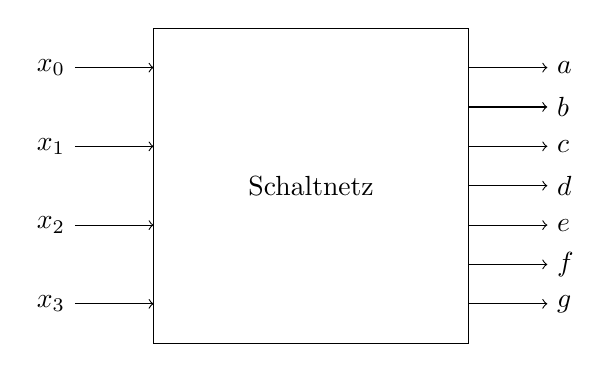
\begin{tikzpicture}
\draw[->] (0,3) node[left]{$x_0$} -- (1,3);
\draw[->] (0,2) node[left]{$x_1$} -- (1,2);
\draw[->] (0,1) node[left]{$x_2$} -- (1,1);
\draw[->] (0,0) node[left]{$x_3$} -- (1,0);

\draw[->] (5,3) -- (6,3) node[right]{$a$};
\draw[->] (5,2.5) -- (6,2.5) node[right]{$b$};
\draw[->] (5,2) -- (6,2) node[right]{$c$};
\draw[->] (5,1.5) -- (6,1.5) node[right]{$d$};
\draw[->] (5,1) -- (6,1) node[right]{$e$};
\draw[->] (5,0.5) -- (6,0.5) node[right]{$f$};
\draw[->] (5,0) -- (6,0) node[right]{$g$};

\draw (1,-0.5) rectangle node {Schaltnetz} (5,3.5);
\end{tikzpicture}
\end{center}

\subex{Wahrheitstafel}
\begin{center}
\begin{ctabular}{CCCC|CCCCCCC}
$x_3$ & $x_2$ & $x_1$ & $x_0$ & a & b & c & d & e & f & g \\ \hline
  0   &   0   &   0   &   0   & 1 & 1 & 1 & 1 & 1 & 1 & 0 \\
  0   &   0   &   0   &   1   & 0 & 1 & 1 & 0 & 0 & 0 & 0 \\
  0   &   0   &   1   &   0   & 1 & 1 & 0 & 1 & 1 & 0 & 1 \\
  0   &   0   &   1   &   1   & 1 & 1 & 1 & 1 & 0 & 0 & 1 \\
  0   &   1   &   0   &   0   & 0 & 1 & 1 & 0 & 0 & 1 & 1 \\
  0   &   1   &   0   &   1   & 1 & 0 & 1 & 1 & 0 & 1 & 1 \\
  0   &   1   &   1   &   0   &\multicolumn{7}{C}{0}      \\
\vdots&\vdots &\vdots &\vdots &\multicolumn{7}{C}{\vdots} \\
\end{ctabular}
\end{center}

\subex{KV-Diagramme \& Schaltfunktionen}

\begin{multicols}{2}
\textbf{a)}

\begin{tikzpicture}
	\matrix (m)[
      nodes={matrix node},
      matrix of nodes,
      inner sep=0pt,
      outer sep=0pt,
      row sep=-.5pt,
      column sep=-.5pt
   ]  {
      1 & 0 & 1 & 0 \\
      1 & 1 & X & X \\
      X & X & X & X \\
      X & X & X & X \\
   };
  
   \draw[|-|] ($(m-1-3.north west) + (0,1.4cm)$) -- node[above] () {$x_2$} ($(m-1-4.north east) + (0,1.4cm)$);
   \draw[|-|] ($(m-1-2.north west) + (0,.6cm)$) -- node[above] () {$x_0$} ($(m-1-3.north east) + (0,.6cm)$);
   \draw[|-|] ($(m-2-1.north west) + (-.6cm,0)$) -- node[left] () {$x_1$} ($(m-3-1.south west) + (-.6cm,0)$);
   \draw[|-|] ($(m-3-1.north west) + (-1.4cm,0)$) -- node[left] () {$x_3$} ($(m-4-1.south west) + (-1.4cm,0)$);
  
   \draw[highlight, dashed] ($(m-1-1.north west) + (3pt,-3pt)$) rectangle ($(m-4-1.south east) + (-3pt,3pt)$);
   \draw[highlight, dashed] ($(m-2-1.north west) + (3pt,-3pt)$) rectangle ($(m-2-4.south east) + (-3pt,3pt)$);
   \draw[highlight, dashed] ($(m-1-3.north west) + (3pt,-3pt)$) rectangle ($(m-4-3.south east) + (-3pt,3pt)$);
\end{tikzpicture}

$a = x_1\comp x_3 + x_0 x_2 + \comp x_0 \comp x_2$


\textbf{b)}

\begin{tikzpicture}
	\matrix (m)[
      nodes={matrix node},
      matrix of nodes,
      inner sep=0pt,
      outer sep=0pt,
      row sep=-.5pt,
      column sep=-.5pt
   ]  {
      1 & 1 & 1 & 0 \\
      1 & 1 & X & X \\
      X & X & X & X \\
      X & X & X & X \\
   };
  
   \draw[|-|] ($(m-1-3.north west) + (0,1.4cm)$) -- node[above] () {$x_2$} ($(m-1-4.north east) + (0,1.4cm)$);
   \draw[|-|] ($(m-1-2.north west) + (0,.6cm)$) -- node[above] () {$x_0$} ($(m-1-3.north east) + (0,.6cm)$);
   \draw[|-|] ($(m-2-1.north west) + (-.6cm,0)$) -- node[left] () {$x_1$} ($(m-3-1.south west) + (-.6cm,0)$);
   \draw[|-|] ($(m-3-1.north west) + (-1.4cm,0)$) -- node[left] () {$x_3$} ($(m-4-1.south west) + (-1.4cm,0)$);
  
   \draw[highlight, dashed] ($(m-1-1.north west) + (3pt,-3pt)$) rectangle ($(m-2-2.south east) + (-3pt,3pt)$);
   \draw[highlight, dashed] ($(m-1-3.north west) + (3pt,-3pt)$) rectangle ($(m-4-3.south east) + (-3pt,3pt)$);
\end{tikzpicture}

$b = x_0 x_2 + \comp x_2 \comp x_3$

\end{multicols}


\subex{Zusatzaufgabe:}

\begin{multicols}{2}
\textbf{a)}

\begin{tikzpicture}
	\matrix (m)[
      nodes={matrix node},
      matrix of nodes,
      inner sep=0pt,
      outer sep=0pt,
      row sep=-.5pt,
      column sep=-.5pt
   ]  {
      1 & 0 & 1 & 0 \\
      1 & 1 & 1 & 1 \\
      1 & 1 & 1 & 1 \\
      1 & 1 & 1 & 1 \\
   };
  
   \draw[|-|] ($(m-1-3.north west) + (0,1.4cm)$) -- node[above] () {$x_2$} ($(m-1-4.north east) + (0,1.4cm)$);
   \draw[|-|] ($(m-1-2.north west) + (0,.6cm)$) -- node[above] () {$x_0$} ($(m-1-3.north east) + (0,.6cm)$);
   \draw[|-|] ($(m-2-1.north west) + (-.6cm,0)$) -- node[left] () {$x_1$} ($(m-3-1.south west) + (-.6cm,0)$);
   \draw[|-|] ($(m-3-1.north west) + (-1.4cm,0)$) -- node[left] () {$x_3$} ($(m-4-1.south west) + (-1.4cm,0)$);
  
   \draw[highlight, dashed] ($(m-1-1.north west) + (3pt,-3pt)$) rectangle ($(m-4-1.south east) + (-3pt,3pt)$);
   \draw[highlight, dashed] ($(m-2-1.north west) + (3pt,-3pt)$) rectangle ($(m-2-4.south east) + (-3pt,3pt)$);
   \draw[highlight, dashed] ($(m-1-3.north west) + (3pt,-3pt)$) rectangle ($(m-4-3.south east) + (-3pt,3pt)$);
   \draw[highlight, dashed] ($(m-3-1.north west) + (3pt,-3pt)$) rectangle ($(m-4-4.south east) + (-3pt,3pt)$);
\end{tikzpicture}

$a = x_1\comp x_3 + x_0 x_2 + \comp x_0 \comp x_2 + x_3$


\textbf{b)}

\begin{tikzpicture}
	\matrix (m)[
      nodes={matrix node},
      matrix of nodes,
      inner sep=0pt,
      outer sep=0pt,
      row sep=-.5pt,
      column sep=-.5pt
   ]  {
      1 & 1 & 1 & 0 \\
      1 & 1 & 0 & 0 \\
      0 & 0 & 0 & 0 \\
      0 & 0 & 0 & 0 \\
   };
  
   \draw[|-|] ($(m-1-3.north west) + (0,1.4cm)$) -- node[above] () {$x_2$} ($(m-1-4.north east) + (0,1.4cm)$);
   \draw[|-|] ($(m-1-2.north west) + (0,.6cm)$) -- node[above] () {$x_0$} ($(m-1-3.north east) + (0,.6cm)$);
   \draw[|-|] ($(m-2-1.north west) + (-.6cm,0)$) -- node[left] () {$x_1$} ($(m-3-1.south west) + (-.6cm,0)$);
   \draw[|-|] ($(m-3-1.north west) + (-1.4cm,0)$) -- node[left] () {$x_3$} ($(m-4-1.south west) + (-1.4cm,0)$);
  
   \draw[highlight, dashed] ($(m-1-1.north west) + (3pt,-3pt)$) rectangle ($(m-2-2.south east) + (-3pt,3pt)$);
   \draw[highlight, dashed] ($(m-1-2.north west) + (3pt,-3pt)$) rectangle ($(m-1-3.south east) + (-3pt,3pt)$);
\end{tikzpicture}

$b = x_0 \comp x_1 \comp x_3 + \comp x_2 \comp x_3$

\end{multicols}
\bigskip

Der qualitative Unterschied ist, dass nun die \emph{don't care}-Terme eine Rolle spielen, also im Grunde keine mehr sind.


\end{document}
